\documentclass[11pt]{article}
\renewcommand{\baselinestretch}{1} 
\usepackage[utf8]{inputenc}
\usepackage[rightcaption]{sidecap}

\usepackage{float}
\usepackage{wrapfig}

\usepackage{natbib}
\usepackage{algorithm}% http://ctan.org/pkg/algorithm
\usepackage{algpseudocode}% http://ctan.org/pkg/algorithmicx
\usepackage{graphicx}
\usepackage{caption}
\usepackage{capt-of}
\usepackage{subcaption}
\usepackage{verbatim}
\usepackage{grffile}
\usepackage[subsection]{placeins}
\usepackage{geometry}
\geometry{
 a4paper,
 left=25mm,
 top=20mm,
 right = 20 mm
 } 

%\floatstyle{boxed} % or whatever
%\restylefloat{figure}

\graphicspath{ {./images/} }
\begin{document}

\begin{titlepage}

\newcommand{\HRule}{\rule{\linewidth}{0.9mm}} % Defines a new command for the horizontal lines, change thickness here

\center % Center everything on the page
\\[0.5cm]
%----------------------------------------------------------------------------------------
%    HEADING SECTIONS
%----------------------------------------------------------------------------------------

\textsc{\Large \textbf{Department of Electronic and Telecommunication
Engineering}\small \\EN 4053 - Digital Communication II}\\[10mm] % Name of your university/college

%----------------------------------------------------------------------------------------
%    LOGO SECTION
%----------------------------------------------------------------------------------------

\includegraphics[ height=5cm]{uomlogo.png}\\[0.1cm]
\textsc{\Large  \textbf{University Of Moratuwa}}\\[0.5cm] 
%----------------------------------------------------------------------------------------
\textsc{\large \\Assignment 2}\\[0cm] % Minor heading such as course title

%----------------------------------------------------------------------------------------
%    TITLE SECTION
%----------------------------------------------------------------------------------------

%\HRule
\\[1cm]
{ \huge \bfseries Error Correction Coding}\\[9cm] % Title of your document
%\HRule 
\\[1cm]
 
%----------------------------------------------------------------------------------------
%    AUTHOR SECTION
%----------------------------------------------------------------------------------------


\emph{\large \textbf{Group Members:}}\\
\begin{tabular}{ll}\large
\large A. L. A. V. \textsc{Isuru}&\tab \large - 140239D\\
\large H.D. \textsc{Fernando}&\tab \large - 140154L\\
\large W.D.A.P. \textsc{Ravinath}&\tab \large - 140530L
\end{tabular}\\[1cm]




% If you don't want a supervisor, uncomment the two lines below and remove the section above
%\Large \emph{Author:}\\
%John \textsc{Smith}\\[3cm] % Your name

%----------------------------------------------------------------------------------------
%    DATE SECTION
%----------------------------------------------------------------------------------------

{\large \today}\\[0.1cm] % Date, change the \today to a set date if you want to be precise



\vfill % Fill the rest of the page with whitespace

\end{titlepage}

\clearpage

%----------------------------------------------------------------------------------------%
%                                     VIJITHA                                            %
%----------------------------------------------------------------------------------------%



\section{Transmission of data over an AWGN channel}
\subsection{Baseband Communication System}
\begin{center}
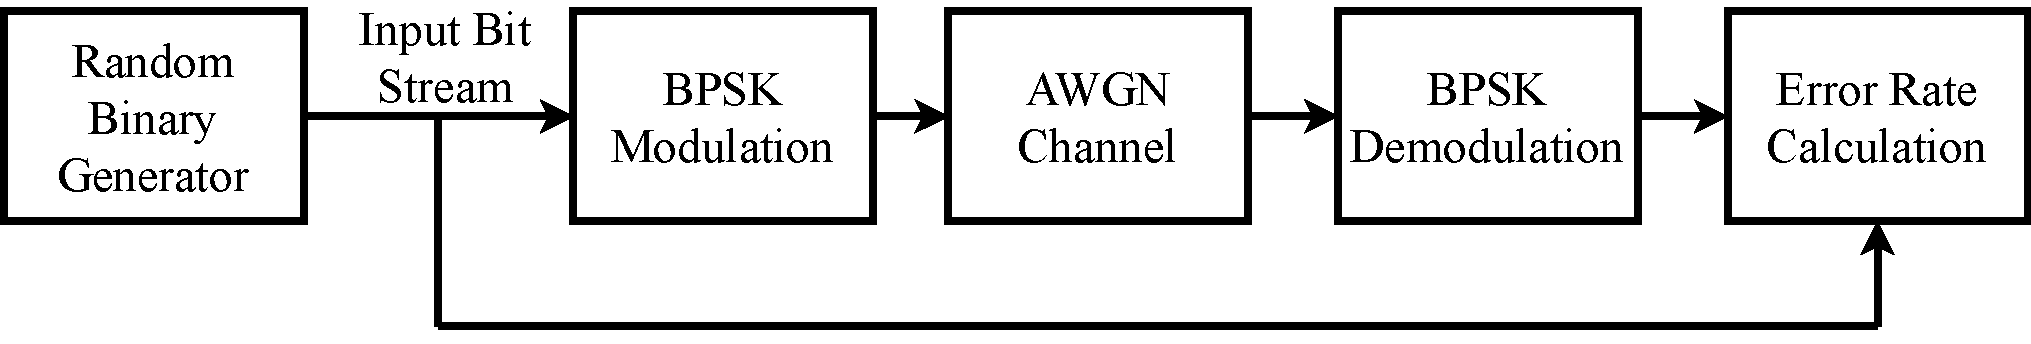
\includegraphics[width=.7\textwidth]{baseband-com-in-awgn-ch.pdf}
\label{fig:baseband-com-sys}
\captionof{figure}{Baseband Communication System in an AWGN Channel}
\end{center}
Answer here.


\subsection{Table 1's answer}

\begin{table}[h]
\centering
\begin{tabular}{|c|c|c|c|c|c|c|c|c|c|}

\hline
$E_{b}/N_{0}$ (dB) & -4 & -2 & 0 & 2 & 4 & 6 & 8 & 10 & 12 \\\hline
$P_{\tau}$ (W) & 0 & 0 & 0 & 0 & 0 & 0 & 0 & 0 & 0 \\\hline             % ***** EDIT HERE *****

\end{tabular}
\caption{\label{tab:transmit_power_levels}Transmit power levels to achieve different $E_{b}/N_{0}$.}
\end{table}

\subsection{Table 1's answer}
Answer
\subsection{Table 1's answer}
Answer
%----------------------------------------------------------------------------------------%
%                                     HESHAN                                             %
%----------------------------------------------------------------------------------------%
\section{Error correction using Hamming codes}
\subsection{Table 1's answer}
Answer
\subsection{Table 1's answer}
Answer
\subsection{Table 1's answer}
Answer
\subsection{Table 1's answer}
Answer
\subsection{Table 1's answer}
Answer

%----------------------------------------------------------------------------------------%
%                                     AMILA                                              %
%----------------------------------------------------------------------------------------%

\section{Error correction using Convolution codes}
\subsection{Build the baseband communication model shown in Figure 4 in Simulink}
\begin{center}
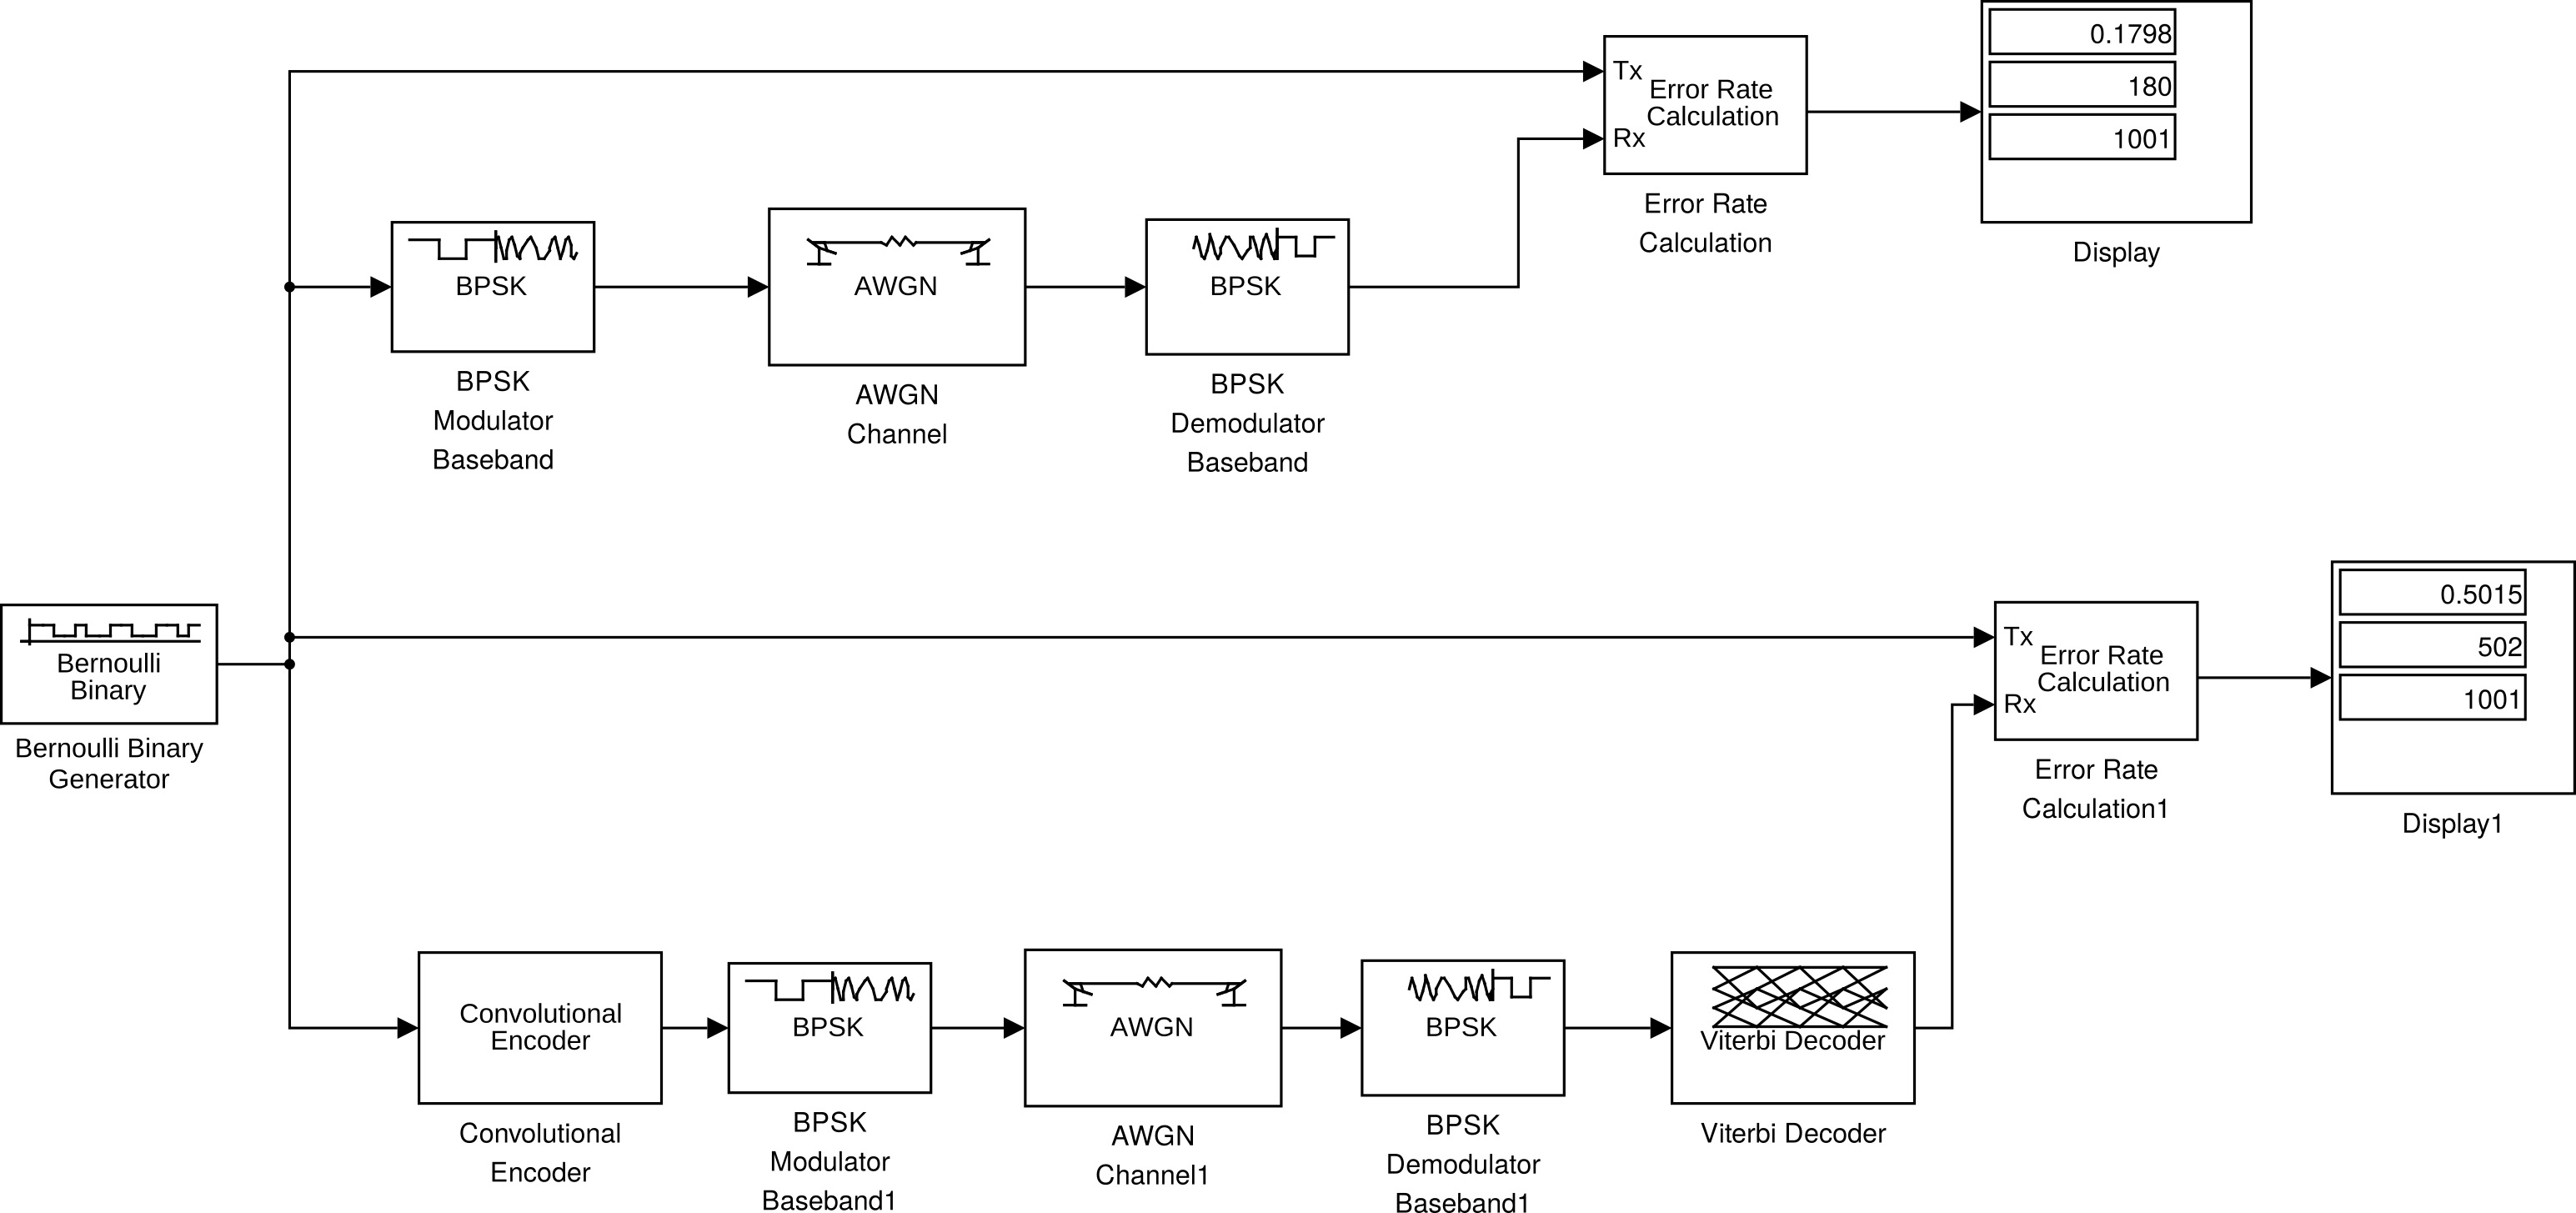
\includegraphics[width=.7\textwidth]{images/q6-model.png}
\label{fig:q6-model}
\captionof{figure}{Baseband communication system with Convolution coder / Viterbi decoder in an AWGN
channel}
\end{center}
\subsection{Carry out the simulation for each $E_b/N_0$ value given in the table 1 separately. Continue your
simulations until you obtain at least 100 bit errors for each $E_b/N_0$ value}
Answer
\subsection{Plot the average BER obtained for uncoded and convolutional coded systems with the
$E_b/N_0$ on the same graph}
Answer
\subsection{Table 1's answer}
Answer

%----------------------------------------------------------------------------------------%
%                                     DISCUSSION                                         %
%----------------------------------------------------------------------------------------%

\section{Discussion}
\subsection{Comment on and explain the BER plots you have obtained for Uncoded, Hamming coded and
convolution coded systems}
Answer
\subsection{Briefly explain the factors required to be taken into consideration in selecting a suitable
channel coding scheme for a given application}
Answer
\bibliographystyle{plain}
\bibliography{references}
\end{document}

 